\documentclass[10pt,a4paper]{article}
\usepackage[left=2cm,right=2cm,top=2cm,bottom=2cm]{geometry}
\usepackage[dvipsnames]{xcolor}
\usepackage[fleqn]{mathtools}
\usepackage{booktabs}
\usepackage{amsmath}
\usepackage{latexsym}
\usepackage{graphicx}
\usepackage{nccmath}
\usepackage{multicol}
\usepackage{listings}
\usepackage{tasks}
\usepackage{color}
\usepackage{float}
\usepackage{longtable}
\usepackage{lipsum}
\usepackage[utf8]{inputenc}
\usepackage[T1]{fontenc}
% \usepackage[spanish]{babel}

\definecolor{colorIPN}{rgb}{0.5, 0.0,0.13}
\definecolor{colorESCOM}{rgb}{0.0, 0.5,1.0}
\graphicspath{ {imagenes/} }

\begin{document}
%#########################################################
\begin{titlepage}
	\centering
	{ \huge \bfseries \color{colorIPN}{Instituto Politécnico Nacional} \par}
	{ \Large \bfseries  \color{colorESCOM}{Escuela Superior de Cómputo} \par }
	\vspace{1cm}
	{\huge\Large \color{colorIPN}{Probability and Statistics research}.\par}
	\vspace{1.5cm}
	{\huge\Large  \color{colorESCOM}{From Statistical Estimation to Bayesian Classification: Modeling Human-AI Interaction}\par}
		\vspace{2cm}
	{\Large\itshape \color{colorIPN}{Professor:Elena Fabiola Ruiz Ledesma }\par} \hfill \break
	\vspace{2cm}
	{\Large\itshape \color{colorIPN}{Alumno: Sánchez Ruiz Leonardo}\par} \hfill \break
	{\Large\itshape \color{colorIPN}{sanchez.ruiz.leonardo9@gmail.com}\par} \hfill \break
	{\Large\itshape \color{colorIPN}{4BM1} \par}
	\vfill
	{\large \color{colorIPN}{\today}\par} 
	\vfill
\end{titlepage}

\renewcommand\lstlistingname{Quelltext} 


\lstset{ 
	language=Java,
	basicstyle=\small\sffamily,
	numbers=left,
	numberstyle=\tiny,
	frame=tb,
	tabsize=4,
	columns=fixed,
	showstringspaces=false,
	showtabs=false,
	keepspaces,
	commentstyle=\color{Violet},
	keywordstyle=\color{colorIPN} \bfseries,
	stringstyle=\color{colorESCOM}
}

\settasks{
	counter-format=(tsk[r]),
	label-width=4ex
}
\tableofcontents 
\pagebreak
\listoffigures
\pagebreak
\listoftables
\pagenumbering {arabic}

\pagebreak

\begin{abstract}

The rapid adoption of conversational artificial intelligence has transformed chatbots from productivity tools into social companions capable of providing emotional support, advice, and personalized interaction. As these systems become increasingly integrated into daily life, concerns have emerged regarding the development of emotional attachment and dependency toward AI.

This study investigates behavioral and emotional dependency toward artificial intelligence among university students using a combination of psychometric validation, statistical inference, and probabilistic machine learning. Data were collected through a questionnaire administered to predominantly university students between 18 and 24 years old. from different academic institutions and social contexts. A dependency score was constructed from six Likert-scale items and analyzed both as a continuous and categorical variable.

The results indicate that students with higher levels of AI usage exhibit significantly greater dependency scores than low-usage users. In contrast, social interaction frequency showed only weak evidence of association with dependency levels. A Categorical Naive Bayes classifier was trained to predict dependency categories from behavioral characteristics, achieving an overall accuracy of 0.86.

These findings suggest that frequency of AI use is a stronger indicator of dependency than social interaction patterns within the studied population. More broadly, the study demonstrates how statistical methods and machine learning can be combined to investigate emerging forms of human-AI relationships and their potential social implications.

\end{abstract}

\section{{\color{colorIPN}{Introduction}}}

Artificial intelligence has become one of the most influential technologies of the last decade, transforming the way individuals communicate, learn, work, and seek information. The emergence of large language models and conversational agents such as ChatGPT, Replika, and Character.ai has expanded the role of AI beyond traditional computational tasks, enabling interactions that increasingly resemble human conversation and social engagement. As a result, users are beginning to form emotional connections with AI systems, sometimes describing these interactions in terms traditionally associated with friendship, companionship, or even romantic attachment \cite{ref1}.

The growing popularity of AI companions reflects a broader shift in the way technology is used in everyday life. Recent reports indicate that emotional support and companionship have become among the most common motivations for interacting with generative AI systems \cite{ref4}. In addition, researchers have highlighted the potential of AI-driven conversational agents to support mental health interventions, improve accessibility to psychological assistance, and provide continuous emotional support \cite{ref5}. These applications suggest that AI may increasingly occupy roles traditionally fulfilled by human relationships and professional support networks.

Despite these potential benefits, the rise of emotionally engaging AI systems has generated significant ethical and psychological concerns. Several highly publicized cases involving harmful interactions with chatbots have raised questions about the responsibilities of AI developers and the potential consequences of prolonged emotional reliance on artificial companions \cite{ref2,ref3}. Concerns regarding emotional dependency, social isolation, trust, and the substitution of human relationships have become increasingly relevant as these technologies continue to evolve.

Although previous studies have explored emotional attachment to AI, mental health applications, and ethical implications, relatively little research has quantitatively examined dependency toward AI among university students. Understanding the factors associated with AI dependency is particularly important for younger populations, who represent some of the most active users of conversational AI systems.

Therefore, this study investigates behavioral and emotional dependency toward artificial intelligence among university students through survey-based statistical analysis and machine learning techniques. Specifically, the research evaluates whether AI usage patterns and social interaction behaviors are associated with dependency levels and explores the predictive value of these behavioral characteristics using a Categorical Naive Bayes classifier.
\pagebreak
\section{{\color{colorIPN}{Literature Review}}}

\subsection{AI as Social and Emotional Companions}

Recent developments in generative artificial intelligence have enabled conversational agents to function as social companions capable of providing emotional support and maintaining long-term interactions with users. Research has shown that individuals frequently attribute human-like characteristics to AI systems, forming emotional bonds that resemble friendship or romantic attachment \cite{ref1}. These interactions blur the distinction between human and machine relationships, creating new forms of social engagement mediated by artificial intelligence.

The increasing prevalence of AI companionship is reflected in user behavior. Recent reports indicate that companionship and emotional connection are among the primary motivations for using large language models, highlighting a shift from purely functional applications toward emotionally meaningful interactions \cite{ref4}. This trend suggests that AI systems are increasingly occupying social roles traditionally fulfilled by other humans.

\subsection{Artificial Intelligence in Mental Health Support}

Artificial intelligence has also gained attention within psychology and psychotherapy. Researchers have explored the use of AI-driven systems to improve access to mental health resources, provide continuous support, and assist in the diagnosis and treatment of psychological disorders \cite{ref5}. Studies have reported positive outcomes in the use of conversational agents for reducing symptoms of anxiety and depression while improving emotional well-being.

These findings suggest that AI-based systems may serve as accessible support tools, particularly for individuals who face barriers to traditional mental health services. However, the increasing reliance on AI for emotional support raises questions regarding the long-term consequences of substituting human interaction with machine-mediated relationships.

\subsection{Risks and Ethical Concerns of Human-AI Relationships}

Alongside the potential benefits of AI companionship, researchers have identified several ethical and psychological concerns. The ability of conversational agents to simulate empathy and emotional understanding may encourage users to develop strong attachments to systems that lack genuine emotions or intentions \cite{ref1}. This ambiguity can create uncertainty regarding trust, authenticity, and the nature of the relationship itself.

Several highly publicized incidents have intensified concerns about the impact of AI companions on vulnerable users. These cases have sparked debates regarding the responsibilities of AI developers and the need for safeguards that prevent harmful interactions \cite{ref2,ref3}. Consequently, understanding the conditions under which dependency may emerge has become an increasingly important area of research.

\subsection{Research Gap}

Although previous studies have explored emotional attachment, mental health applications, and ethical concerns surrounding AI companions, limited research has quantitatively examined how AI usage behavior and social interaction patterns relate to dependency levels among university students. Most existing work focuses on conceptual, clinical, or ethical perspectives rather than statistical analysis of behavioral data.

This study seeks to address this gap by combining survey-based measurement, statistical hypothesis testing, and probabilistic machine learning techniques to investigate factors associated with AI dependency and to evaluate the predictive value of behavioral characteristics.

\pagebreak

\section{{\color{colorIPN}{Research Method}}}
Data was collected through a structured questionnaire designed to evaluate behavioral and emotional dependency toward artificial intelligence systems. The survey collected 140 responses, primarily from university students. Most participants (78.7\%) were between 18 and 21 years old, while smaller proportions belonged to the 22--24, over-25, and under-18 age groups. Participants were recruited from different academic institutions, including students from urban universities as well as a subset from semi-rural areas. This sampling diversity may have influenced the observed distribution of AI usage and dependency levels, potentially contributing to a higher proportion of low-usage and low-dependency responses.

The instrument consisted of 15 questions in total. Six of these items were measured using a 5-point Likert scale and were specifically designed to assess emotional reliance, trust, and behavioral attachment toward artificial intelligence systems. The remaining items were categorical in nature and captured demographic, behavioral, and usage-related characteristics.

To ensure the reliability of the measurement instrument, internal consistency was evaluated using Cronbach's alpha. The coefficient was computed as:

\[
\alpha =
\frac{k}{k-1}
\left(
1 - \frac{\sum_{i=1}^{k} \sigma_i^2}{\sigma_T^2}
\right)
\]

where $k$ is the number of items, $\sigma_i^2$ is the variance of each item, and $\sigma_T^2$ is the variance of the total score.

The obtained value of Cronbach's alpha was:

\[
\alpha = 0.869
\]

indicating good internal consistency of the questionnaire.

A dependency score was constructed by averaging the responses of the six Likert-scale items. This score was treated both as a continuous variable for statistical analysis and as a categorical variable by discretizing it into three levels: low, medium, and high dependency.
\begin{figure}[H]
    \centering
    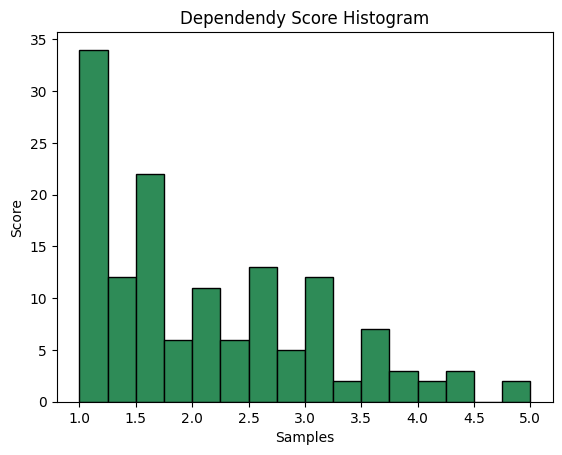
\includegraphics[width=0.75\textwidth]{dependency_histogram.png}
    \caption{Distribution of dependency score of sample}
\end{figure}

\pagebreak
\subsection{Confidence Interval for the Mean Dependency Score}

To estimate the population mean of the dependency score, a 95\% confidence interval was computed using the t-distribution:

\[
\bar{x} \pm t_{\alpha/2} \cdot \frac{s}{\sqrt{n}}
\]

where:
\begin{itemize}
    \item $\bar{x}$ is the sample mean
    \item $s$ is the sample standard deviation
    \item $n$ is the sample size
    \item $t_{\alpha/2}$ is the critical t-value for $n-1$ degrees of freedom
\end{itemize}

The resulting confidence interval for the mean dependency score was:

\[
CI_{95\%} = [\text{1.92}, \text{2.26}]
\]

This interval provides an estimate of the range in which the true population mean dependency level is expected to lie.

\subsection{Independent Samples t-Test}

To evaluate whether high AI usage is associated with higher dependency levels, an independent samples t-test was conducted comparing the mean dependency scores between high-usage and low-usage users.

The null and alternative hypotheses were defined as:

\[
H_0: \mu_1 = \mu_2
\]

\[
H_1: \mu_1 > \mu_2
\]

where $\mu_1$ represents the mean dependency score of high-usage users and $\mu_2$ represents the mean dependency score of low-usage users.

Under the null hypothesis, the difference between sample means is expected to be zero. By the Central Limit Theorem, the sampling distribution of the difference of means approximates normality for sufficiently large sample sizes.

The test statistic was computed using Welch’s t-test:

\[
t =
\frac{\bar{x}_1 - \bar{x}_2}
{
\sqrt{
\frac{s_1^2}{n_1} +
\frac{s_2^2}{n_2}
}
}
\]

where:
\begin{itemize}
    \item $\bar{x}_1$ and $\bar{x}_2$ are the sample means
    \item $s_1^2$ and $s_2^2$ are the sample variances
    \item $n_1$ and $n_2$ are the sample sizes
\end{itemize}

The resulting p-value obtained from the test was:

\[
p = 0.003
\]

Using a significance level of $\alpha = 0.05$, the null hypothesis was rejected, indicating statistically significant evidence that high-usage users exhibit higher dependency scores.

\begin{figure}[H]
    \centering
    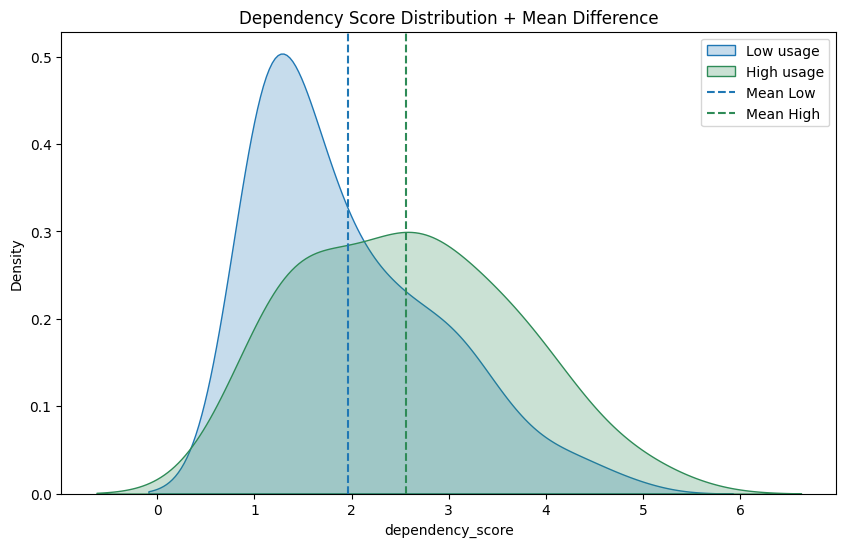
\includegraphics[width=0.75\textwidth]{t_test_distribution.png}
    \caption{Distribution of dependency scores between low and high AI usage groups}
\end{figure}

\subsection{Chi-Squared Test of Independence}

To examine the relationship between social interaction frequency and dependency level, a chi-squared test of independence was performed.

The hypotheses were defined as:

\[
H_0: \text{Social Interaction and AI Dependency are independent}
\]

\[
H_1: \text{Social Interaction and AI Dependency are associated}
\]

The chi-squared statistic is defined as:

\[
\chi^2 = \sum \frac{(O - E)^2}{E}
\]

where $O$ represents observed frequencies and $E$ represents expected frequencies under independence.

The test yielded a p-value of:

\[
p = 0.053
\]

At a significance level of $\alpha = 0.05$, we fail to reject the null hypothesis; however, the result suggests a weak association between social interaction frequency and AI dependency, indicating a potential relationship that may require further investigation with a larger sample size.

\begin{figure}[H]
    \centering
    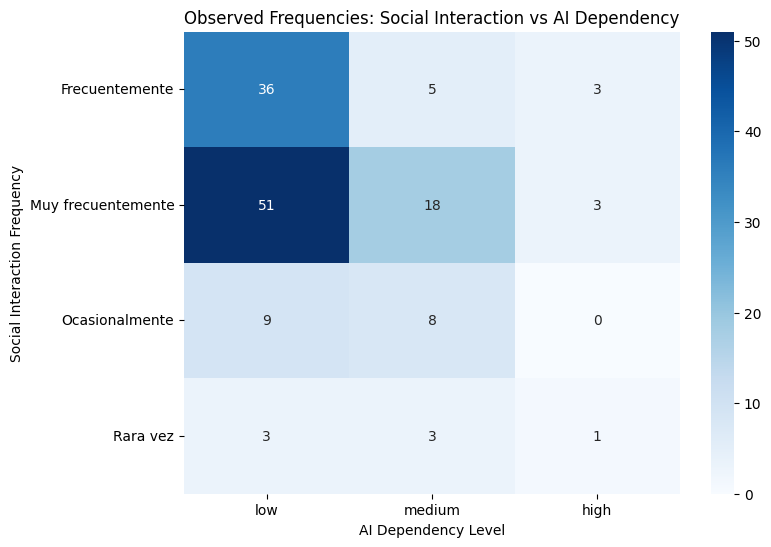
\includegraphics[width=0.75\textwidth]{chi_square_heatmap.png}
    \caption{Observed frequency distribution between social interaction and AI dependency}
\end{figure}

\subsection{Naive Bayes Model}

To model the relationship between behavioral features and AI dependency levels, a Naive Bayes classifier was employed. This model is grounded in Bayes' theorem, which describes the conditional probability of a class given observed features.

\[
P(Y \mid X) = \frac{P(X \mid Y)\,P(Y)}{P(X)}
\]

where:
\begin{itemize}
    \item $Y$ represents the dependency class (low, medium, high)
    \item $X$ represents the observed feature vector
\end{itemize}
In this context, the model estimates the probability of a given dependency level based on behavioral and social features such as AI usage frequency, social interaction, and preference for AI-based advice.
The Naive Bayes classifier assumes conditional independence between features given the class label. This simplifies the joint likelihood as:

\[
P(X \mid Y) = \prod_{i=1}^{n} P(x_i \mid Y)
\]

where each feature $x_i$ is assumed to contribute independently to the probability of the class $Y$.
Although this assumption is rarely strictly true in real-world behavioral data, it provides a computationally efficient and surprisingly effective approximation for classification problems.
The final classification is obtained by selecting the class with the highest posterior probability:

\[
\hat{Y} = \arg\max_Y \; P(Y) \prod_{i=1}^{n} P(x_i \mid Y)
\]
In this study, the feature vector $X$ consists of encoded behavioral variables including AI usage frequency, social interaction level, emotional support from AI, and preference for AI-based advice. All features were discretized to enable the use of a categorical Naive Bayes classifier.
The Naive Bayes model provides a probabilistic framework to classify individuals into dependency levels based on observed behavioral patterns. Rather than modeling causal relationships, it captures statistical associations between features and dependency categories.

\section{{\color{colorIPN}{Results and Discussion}}}
The analysis combines statistical inference and probabilistic classification to study behavioral patterns related to AI dependency. A dependency score was constructed from the average of six Likert-scale items and treated both as a continuous variable for statistical testing and as a categorical variable for classification purposes.

To evaluate differences in dependency levels between usage groups, an independent samples t-test was conducted. The results showed a statistically significant difference in mean dependency scores between high-usage and low-usage users (p = 0.003), suggesting that increased AI usage is associated with higher dependency levels.

In contrast, the chi-squared test of independence between social interaction frequency and dependency level produced a marginal result (p = 0.053). Although not statistically significant at the 0.05 level, the observed distribution suggests a weak association that may become clearer with a larger sample size. Overall, these results indicate that AI usage is a stronger predictor of dependency than social interaction patterns within this dataset.

A Categorical Naive Bayes classifier was then trained to predict dependency levels based on behavioral and demographic features. The model achieved moderate performance, with stronger predictive ability for the low dependency class compared to medium and high levels. This behavior is also reflected in the confusion matrix, which shows a tendency to classify observations as low dependency more frequently. This pattern is consistent with the underlying class distribution and the ambiguity of the medium category, rather than being solely a model limitation.
\begin{figure}[H]
    \centering
    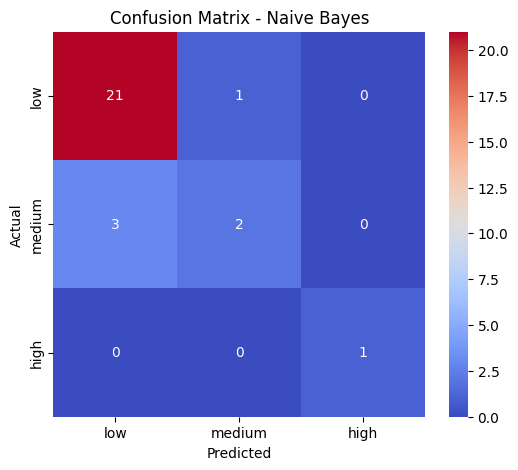
\includegraphics[width=0.75\textwidth]{confusion_matrix.png}
    \caption{Confusion Matrix}
\end{figure}


The performance of the classifier is summarized in the table below:

\begin{table}[H]
\centering
\begin{tabular}{c|c|c|c|c}
Class & Precision & Recall & F1-score & Support \\
\hline
0 (Low)    & 0.88 & 0.95 & 0.91 & 22 \\
1 (Medium) & 0.67 & 0.40 & 0.50 & 5 \\
2 (High)   & 1.00 & 1.00 & 1.00 & 1 \\
\hline
Accuracy & \multicolumn{4}{c}{0.86} \\
Macro Avg & 0.85 & 0.78 & 0.80 & 28 \\
Weighted Avg & 0.84 & 0.86 & 0.84 & 28 \\
\end{tabular}
\caption{Performance metrics of the Naive Bayes classifier}
\end{table}

Overall, the model achieved an accuracy of 0.86 (The classifier correctly identified 24 out of 28 test observations), indicating good general performance in classifying dependency levels. However, performance varies across classes. The model performs best for low dependency cases, while medium dependency cases are often misclassified as low, indicating lower recall for this category. The high dependency class shows perfect scores, although this is not statistically reliable due to the extremely small number of samples.

The difference between macro and weighted averages further highlights the presence of class imbalance, with the model being biased toward the majority class (low dependency).

Finally, the results suggest that while AI usage frequency is significantly associated with dependency levels, social interaction shows only weak evidence of association. The Naive Bayes model confirms that behavioral features contain predictive signal, but also reflects limitations introduced by class imbalance and overlapping behavioral patterns.

Additionally, the sampling context, which includes both urban and semi-rural participants, may have influenced the distribution of responses, potentially contributing to a higher proportion of low usage and low dependency observations.

Overall, this study highlights both the potential and limitations of combining statistical inference and machine learning techniques to analyze human-AI behavioral dependency.
\section{{\color{colorIPN}{Conclusion}}}

This study examined behavioral and emotional dependency toward artificial intelligence among university students through a combination of psychometric validation, statistical inference, and probabilistic machine learning. By constructing a dependency score from multiple Likert-scale items, the research provided a quantitative framework for analyzing human-AI attachment and usage patterns.

The findings indicate that AI usage frequency is significantly associated with higher dependency levels, suggesting that prolonged interaction with conversational AI systems may contribute to stronger emotional or behavioral reliance. In contrast, social interaction frequency showed only limited evidence of association with dependency, indicating that AI usage behavior may be a more relevant factor than offline social activity within the studied population.

The Categorical Naive Bayes classifier further demonstrated that behavioral characteristics contain predictive information regarding dependency levels. Although the model achieved good overall accuracy, its performance was affected by class imbalance and overlap between categories, highlighting the challenges of modeling complex human behaviors using survey-based data.

Taken together, these results contribute to the growing body of research on human-AI relationships by providing empirical evidence of the connection between AI usage and dependency. As conversational AI systems continue to become integrated into education, work, and personal life, understanding the factors that influence emotional attachment and reliance on these technologies will become increasingly important.

Future research should consider larger and more diverse populations, longitudinal data collection, and additional psychological variables to better understand how dependency toward AI develops over time and how it may influence social behavior, well-being, and interpersonal relationships.
\pagebreak
\begin{thebibliography}{99}

\bibitem{ref1}
R. Zhang and L. Xie, ``The Fragility of AI Companionship: Ontological, Structural, and Normative Uncertainty in Human-AI Relationships,'' \textit{arXiv preprint arXiv:2605.03367}, 2026.

\bibitem{ref2}
C. Voinea, C. Register, S. P. Mann, J. Savulescu, and B. D. Earp, ``The Sorrows of Young Chatbot Users: Harm and Responsibility in Human-AI Relationships,'' \textit{Topoi}, pp. 1--14, 2026.

\bibitem{ref3}
H. Ahmed Kausar, ``Inteligencia Artificial y Afectividad Simulada: Orientaciones para el Tratamiento Informativo Responsable de las Relaciones Parasociales con Chatbots,'' Master's Thesis, Universitat Autònoma de Barcelona, 2025.

\bibitem{ref4}
E. Andoh, ``AI Chatbots and Digital Companions Are Reshaping Emotional Connection,'' \textit{Monitor on Psychology}, vol. 57, no. 1, pp. 1--2, 2026.

\bibitem{ref5}
L. Spytska, ``The Use of Artificial Intelligence in Psychotherapy: Development of Intelligent Therapeutic Systems,'' \textit{BMC Psychology}, vol. 13, no. 1, p. 175, 2025.

\end{thebibliography}

\pagebreak

%################################################

\end{document}
